\documentclass[conference]{IEEEtran}
\usepackage{amsmath,amssymb}
\usepackage{booktabs}
\usepackage{graphicx}
\usepackage{microtype}
\usepackage[hidelinks]{hyperref}
\graphicspath{{figures/}}

\title{Supplementary Material for ``CREATE: A Closed-Loop Reward Editing Agent with Training Evidence for Reinforcement Learning''}
\author{Anonymous Authors}

\begin{document}
\maketitle

\section{Detailed Experimental Protocol}
Each reward candidate trains a freshly initialized PPO policy. LunarLander-v3 uses $10^6$ environment steps, four vectorized environments, 20 fixed search-evaluation episodes, and a native-fitness threshold of 200. BipedalWalker-v3 uses $5\times10^6$ steps and a threshold of 300. Every condition contains five seeds and at most ten complete reward evaluations. The generated reward is used only for policy optimization; candidate selection and reporting use the unmodified environment-native episodic return. Selected reward--policy pairs are evaluated for 100 episodes with seeds not exposed during search.

All main comparisons use DeepSeek V4 Pro with the same environment facts, initial reward-generation interface, code validator, PPO settings, and maximum number of trained reward programs. The methods differ only in candidate dependence, accessible evidence, persistent state, and reward-editing constraints. Exact system prompts, model parameters, API provider, run dates, token usage, wall-clock time, and hardware identifiers should be inserted here from the frozen run manifests before submission.

\section{Compared Conditions}
\textbf{Single-shot generation} evaluates the first reward only. \textbf{Independent-10} trains ten unrelated initial rewards and selects the largest search fitness. \textbf{Stateless iterative revision} receives the current reward and current-round basic feedback but has no tool-organized evidence, persistent intervention memory, cross-round component comparison, hierarchical semantic edit policy, or best-reward context. \textbf{CREATE w/o evidence enrichment} disables the evidence-organizing subagent and processed component diagnostics while retaining memory and hierarchical semantic editing. \textbf{CREATE w/o hierarchical semantic editing} retains enriched evidence, memory, and the best archive but permits free multi-component revision. \textbf{CREATE} uses the complete loop.

\section{Complete LunarLander Search Traces}
The following tables reproduce the rounded search-fitness values used to design the main-paper plots. Final numerical tables should be regenerated directly from the unrounded JSON logs.

\begin{table*}[t]
\caption{Stateless iterative revision. Bold entries are lineage-wise maxima.}
\centering
\scriptsize
\resizebox{\textwidth}{!}{%
\begin{tabular}{lrrrrrrrrrrr}
\toprule
Seed & 1 & 2 & 3 & 4 & 5 & 6 & 7 & 8 & 9 & 10 & Best\\
\midrule
0 & \textbf{25} & -99 & -394 & -353 & -91 & -28 & -123 & -123 & -118 & -119 & 25\\
1 & -84 & -114 & -186 & -113 & -116 & -59 & \textbf{-5} & -113 & -126 & -7 & -5\\
2 & -109 & -65 & -80 & -92 & -72 & -108 & -24 & -68 & \textbf{-10} & -119 & -10\\
3 & \textbf{151} & -27 & -33 & -159 & -47 & -88 & -134 & -115 & -132 & -627 & 151\\
4 & \textbf{59} & -118 & -119 & -116 & -115 & -124 & -122 & -119 & -90 & -72 & 59\\
\bottomrule
\end{tabular}}
\end{table*}

\begin{table*}[t]
\caption{CREATE. A dash denotes stopping after the task was solved or after the configured post-solution criterion.}
\centering
\scriptsize
\resizebox{\textwidth}{!}{%
\begin{tabular}{lrrrrrrrrrrr}
\toprule
Seed & 1 & 2 & 3 & 4 & 5 & 6 & 7 & 8 & 9 & 10 & Best\\
\midrule
0 & -70 & -129 & -26 & -120 & -124 & -18 & -389 & \textbf{224} & -612 & -- & 224\\
1 & -43 & -18 & 28 & -29 & 120 & -17 & 24 & -31 & 168 & \textbf{241} & 241\\
2 & -18 & \textbf{220} & 107 & -- & -- & -- & -- & -- & -- & -- & 220\\
3 & -20 & 148 & -15 & \textbf{254} & 249 & 247 & -- & -- & -- & -- & 254\\
4 & 140 & 114 & \textbf{206} & 206 & 110 & -- & -- & -- & -- & -- & 206\\
\bottomrule
\end{tabular}}
\end{table*}

\begin{table*}[t]
\caption{CREATE without hierarchical semantic editing.}
\centering
\scriptsize
\resizebox{\textwidth}{!}{%
\begin{tabular}{lrrrrrrrrrrr}
\toprule
Seed & 1 & 2 & 3 & 4 & 5 & 6 & 7 & 8 & 9 & 10 & Best\\
\midrule
0 & -122 & 108 & -121 & 14 & -118 & 16 & 16 & -115 & -115 & \textbf{170} & 170\\
1 & -108 & -40 & -63 & \textbf{131} & -119 & -64 & -142 & -- & -- & -- & 131\\
2 & -112 & -21 & \textbf{71} & -8 & -70 & -139 & -120 & -25 & -205 & -296 & 71\\
3 & -10 & -64 & -21 & -123 & -104 & -123 & -122 & -5511 & -5511 & \textbf{59} & 59\\
4 & -102 & -111 & 0 & \textbf{140} & -126 & -79 & 12 & -59 & -116 & -83 & 140\\
\bottomrule
\end{tabular}}
\end{table*}

\begin{table*}[t]
\caption{CREATE without evidence enrichment.}
\centering
\scriptsize
\resizebox{\textwidth}{!}{%
\begin{tabular}{lrrrrrrrrrrr}
\toprule
Seed & 1 & 2 & 3 & 4 & 5 & 6 & 7 & 8 & 9 & 10 & Best\\
\midrule
0 & -110 & -74 & -583 & 46 & -14 & 111 & 145 & \textbf{240} & 216 & -108 & 240\\
1 & 40 & \textbf{170} & -9 & 110 & 34 & 35 & -115 & -138 & -95 & -80 & 170\\
2 & -285 & -298 & -125 & -123 & -125 & -122 & -111 & \textbf{-110} & -110 & -111 & -110\\
3 & -17 & \textbf{116} & -17 & -25 & -114 & -2471 & 2 & -123 & 114 & 115 & 116\\
4 & -19 & -38 & 177 & 180 & 89 & 25 & 256 & \textbf{260} & 21 & -- & 260\\
\bottomrule
\end{tabular}}
\end{table*}

\begin{table*}[t]
\caption{Independent-10. Columns denote unrelated initial candidates rather than revision rounds.}
\centering
\scriptsize
\resizebox{\textwidth}{!}{%
\begin{tabular}{lrrrrrrrrrrr}
\toprule
Seed & 0 & 1 & 2 & 3 & 4 & 5 & 6 & 7 & 8 & 9 & Best\\
\midrule
0 & -105 & -116 & \textbf{-13} & -121 & -125 & -116 & -121 & -21 & -123 & -119 & -13\\
1 & -123 & -121 & -121 & -122 & -115 & -25 & -115 & -123 & -120 & \textbf{171} & 171\\
2 & -118 & -121 & -119 & -47 & -107 & -122 & -122 & \textbf{55} & -124 & -109 & 55\\
3 & -122 & -117 & -123 & -121 & -117 & -119 & -120 & -112 & \textbf{-107} & -113 & -107\\
4 & -118 & -125 & -112 & -115 & -115 & \textbf{-110} & -113 & -117 & -117 & -120 & -110\\
\bottomrule
\end{tabular}}
\end{table*}

\section{Representative Repair Patterns}
The three main-paper traces illustrate distinct successful repair patterns. Seed~0 undergoes collapse and recovery: a differential progress signal fails to supply stable landing guidance at round~7, and an L2 return to state-based proximity with altitude-based anti-exploitation raises fitness to 224 at round~8. Seed~3 exhibits progressive convergence: potential-difference approach shaping first raises fitness to 148, and a later L2 contact refactor supplies a reachable gradient from single-leg to stable two-leg contact, yielding 254. Seed~4 exposes proxy misalignment: a near-ground transition reward is triggered roughly 75 times per episode during bouncing, and an L2 persistent contact-quality gate suppresses the proxy and yields 206.

These cases should be interpreted as diagnostic traces rather than three independent mechanism ablations. Their common structure is that component-level evidence identifies one principal semantic defect and the reward editor applies a localized L2 intervention.

\section{Component-Evidence Heatmaps}
For component $i$, the activation rate is the fraction of logged training steps at which its value is nonzero. A value near zero indicates that the term is effectively unreachable under the current policy, whereas a value near one indicates nearly continuous signaling. The magnitude share is the component's absolute contribution divided by the summed absolute contribution of all logged components. A large share indicates that one term dominates the shaped objective, even when its semantic meaning is only a proxy for task success.

\begin{figure*}[t]
\centering
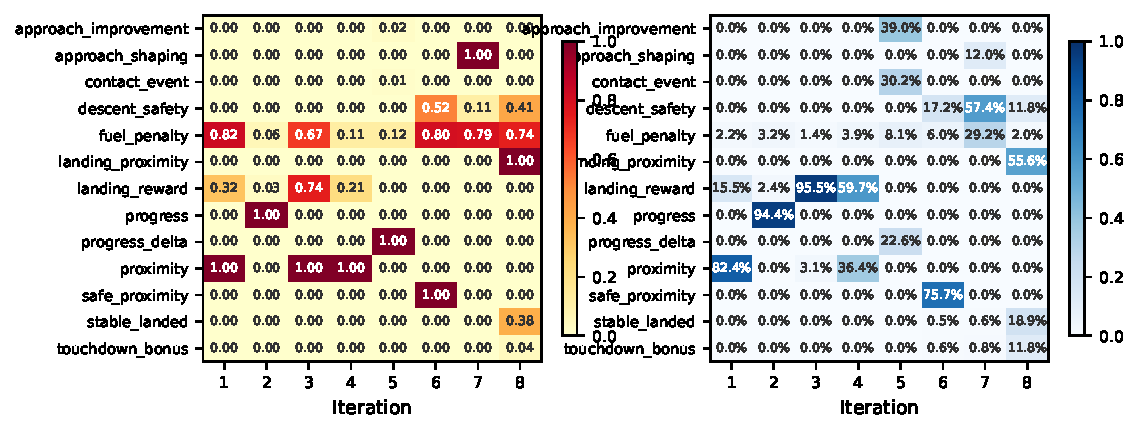
\includegraphics[width=0.92\textwidth]{figS1_seed0_heatmaps.pdf}
\caption{Component evidence for CREATE seed~0. Activation-rate and magnitude-share heatmaps show how component reachability and relative reward scale evolve across reward versions. The round-7 to round-8 transition is interpreted together with the saved reward-code diff and editor decision, rather than from native fitness alone.}
\label{fig:supp_seed0_heatmaps}
\end{figure*}

Fig.~\ref{fig:supp_seed0_heatmaps} provides the detailed evidence behind the seed-0 case in the main paper. The heatmaps indicate which landing-related terms remain inactive, which shaping term controls most of the generated reward, and how those relationships change after the decisive L2 repair. They are descriptive observations supplied to the reward editor, not deterministic rules that directly choose the code modification. Analogous seed-3 and seed-4 heatmaps are included in the released figure artifacts.

\section{Reproducibility and Cost Reporting}
The released supplement should report total trained candidates, total environment steps, LLM calls by role, input/output tokens, wall-clock time, hardware, and peak simultaneous candidate jobs. PPO's four vectorized environments are internal to one candidate-training job and should not be counted as four simultaneous reward candidates. Provider-specific model identifiers and routing settings should be frozen rather than using a moving ``latest'' alias.

\end{document}
